\documentclass[ebook,11pt] {kth-mag}
\usepackage{float}
\usepackage[T1]{fontenc}
\usepackage{textcomp}
\usepackage{lmodern}
\usepackage[latin1]{inputenc}
\usepackage[swedish,english]{babel}
\usepackage{nada-ex}
\usepackage{amsmath}
\usepackage{bm}
\usepackage{babel}
\usepackage{mathtools}
\usepackage{hyperref}


\DeclarePairedDelimiter\ceil{\lceil}{\rceil}
\DeclarePairedDelimiter\floor{\lfloor}{\rfloor}
\title{An optimization approach to the multi-player pursuit-evasion problem}
\subtitle{}
% \author[1]{Yue Jiao 111111-1111 yuejiao@kth.se}	\author[2]{Skvortsov, Ivan 941016-7713 ivansk@kth.se}
\author{
  Jiao, Yue\\
  \texttt{yj@kth.se}
  \\ 
  Skvortsov, Ivan\\
  \texttt{ivansk@kth.se}
}


\date{May 2017}
\blurb{Bachelor's Thesis at the Institution of Mathematics \\
Supervisor: Xiaoming Hu, Silun Zhang\\Examiner: Xiaoming Hu}
\trita{}
\begin{document}
\frontmatter
\maketitle
%%
%% This is file `kth-abs.tex',
%% generated with the docstrip utility.
%%
%% The original source files were:
%%
%% kthesis.dtx  (with options: `abstract')
%% 
%% IMPORTANT NOTICE:
%% 
%% For the copyright see the source file.
%% 
%% Any modified versions of this file must be renamed
%% with new filenames distinct from kth-abs.tex.
%% 
%% For distribution of the original source see the terms
%% for copying and modification in the file kthesis.dtx.
%% 
%% This generated file may be distributed as long as the
%% original source files, as listed above, are part of the
%% same distribution. (The sources need not necessarily be
%% in the same archive or directory.)
\begin{abstract}
  In this paper a scenario of one evader being chased  by multiple pursuers in two specific simulation environments is studied. The simulation environments are divided into an open area without obstacles and a closed area with obstacles. In the open
area a fairly accurate system of dynamics are implemented for both pursuers and evader. The Virtual Vehicle Approach is used to provide a reference trajectory for the pursuers to follow in order to catch the evader. The main purpose of this thesis is to find a decentralized robust
control method for the dynamics of the pursuers. In the closed area, the line of sight and field of view
are introduced and the solution to the Minimum time UGV surveillance problem and the Centroidal
Voronoi partitions. Different
capturing strategies, encirclement and one-on-one chase, are both studied and compared. The
numerical implementation and the resulting simulation are presented and analyzed. Conclusion on
the optimal formation for the multiple pursuers is made.
\end{abstract}
\endinput
%%
%% End of file `kth-abs.tex'.

\clearpage
\selectlanguage{English}
% \begin{abstract}
%   Denna fil ger ett avhandlingsskelett.
%   Mer information om \LaTeX-mallen finns i
%   dokumentationen till paketet.
% \end{abstract}
\selectlanguage{English}
\clearpage
\tableofcontents
\mainmatter
\chapter{Introduction}

\section{Background}
The early versions of the pursuit and evasion problem consisted of mathematical models describing human conflicts and cooperation within a competitive situation, also known as game theory \cite{gametheory}. Game theory can be interpreted as the science of strategy as it helps to explain how to interact in key decision-making moments \cite{bbc}. The concept was founded by J. von Neumann and later introduced to the public after he and his co-writer O. Morgenstern wrote the theory of games \cite{111}. Essentially the book established a foundation for modern game theory and the pursuit-evasion problem. It is seen as one of the major scientific achievements of the first half of the twentieth century, according to A. H. Copeland \cite{222}. 

The pursuit and evasion problem is generally described as a situation where one or a group of pursuers try to catch a moving target or targets, so called evaders. This definition originated from a separate branch of game theory developed in the 1960's, namely Differential Games \cite{333}. The book displayed a group of problems, including pursuit evasion problems such as the Princess and Monster Game \cite{pandm}. The author R. Isaacs also suggested different solutions, including first building a map of the game terrain with boundary conditions. This approach is also used in this report to create a simulation environment.

However, due to the recent technology development has it been made possible to achieve control of more complex pursuit and evasion situations. Solutions have been found for different versions of the original problem and have been a crucial aspect for a wide range of products. These products are most commonly found in the militaristic sector, where for instance fighter aircrafts such as Saab JAS 39 Gripen use sensors to track multiple priority targets \cite{jas}. 

\section{Objective}
The main purpose of this report is to use the control algorithms given by \cite{vva} and to optimize a scenario where a given number of pursuers try to surround an evader. A reference point is chosen on a virtual circle around the evader that moves in the same trajectory as the evader. Each pursuers goal is to reach one of the before mentioned reference points. Each added pursuer creates an additional reference point on the virtual circle. The simulation stops when the pursuers have successfully surrounded the evader at an equal angle between the pursuers. These methods have, to the best of the authors knowledge not been used in this context before. The before mentioned scenario will be split up into two separate simulations. 

\subsection{Open space}
The initial open space problem consists of a defined amount of simulation subjects on a fixed two dimensional linear space with boundary conditions. The subjects have their own heuristically chosen strategies regarding their behavior in the simulation environment. The strategies for both pursuer and evader are thoroughly described in the Method section below. The goal for this fundamental problem is to learn how to properly implement the control algorithms from \cite{vva} and to simulate them. 

\subsection{Closed space}

The second simulation takes place in a more realistic environment. The new map consists of a couple random shaped obstacles that both pursuer and evader can't pass through which are within a defined bounded region. In this case an empirically chosen weight function is used to guide the pursuers to the before mentioned reference points which have the greatest weights. The pursuers also use the method Coverage control given by \cite{sui} to locate the points. The goal of this simulation is to minimize the simulation time by finding an optimal strategy for the pursuer. As for the evader, it will use two strategies. One where the coverage control method is used and the other where it seeks to locate and hide at the furthest hiding spot from the pursuers. In comparison to the open space problem the acceleration of the experiment subjects have been neglected with the purpose of simplicity.

\chapter{Theory and method}
In this part of the paper, the theories and methods used for solving the multi-player pursuit-evasion problem and the numerical simulation are presented. The problem is divided into two separate parts, pursuit-evasion in open space without obstacles and pursuit-evasion in closed space with obstacles. Dynamics of both pursuers and evader is emphasized in the open space. A second order of dynamics is implemented and the method is focused on how each agent follow a reference trajectory with a limited dynamical ability. In the closed space the optimization method for locating and pursuing the evader is studied. The dynamics are reduced to a first order system without consideration for the angular velocity. 

The simulation ends when the evader is successfully captured or when 100 seconds have passed which is considered as a successful escape for the evader. The evader is captured when the pursuers form a regular polygon around the evader on a predefined distance, also the distance between the pursuers must be the same. In the simulation environment the capturing condition is  implemented as a circle which has reference points for the pursuers to follow. This is the same virtual circle as mentioned before. The reference points are placed with an equal arc between them and ultimately form the before mentioned polygon.  

\section{Open space}
\subsection{Assumption}
The simulation environment is considered as a two-dimensional flat surface with infinite size. Both pursuers and evader have second order dynamics, which means that the maximum velocities, accelerations, angular velocities and angular accelerations are known beforehand. The situation of multiple pursuers and a single evader is considered. All agents are considered as stiff bodies with a defined location and a moving direction. 


All pursuers have the same dynamics parameters. From this point they will be called $v_p$ - velocity, $a_p$ - acceleration, $\omega_p$ - angular velocity and $\alpha_p$ - angular acceleration. The corresponding parameters for the evader are called, $v_e$, $a_e$, $\omega_e$ and $\alpha_e$. The evader is assumed to have a lower maximum velocity than the pursuers but  higher acceleration, angular velocity and angular acceleration. 
In mathematical terms: 
$$
v_p > v_e, a_p < a_e, \omega_p < \omega_e, \alpha_p <  \alpha_e
$$

In this report, pursuers and evader are assumed to have different reaction time as well. The evader is assumed to have a faster reaction time. The reaction time is defined as the amount of time the agent spends on making a decision about updating its direction and/or dynamics. The numerical implementation of reaction time is done by updating the agent's dynamics when the time passed is a integer multiple of the agent's reaction time. 

\subsection{Dynamics and the numerical implementation}
To calculate the distance traveled within a short time element $dt$, the following assumption about dynamics can be made. First of all the changes in direction and the magnitude of velocity do not happen simultaneously. But instead, the change of direction happens before the change of velocity. This assumption is made mainly to simplify the simulation. Since the dynamics is assumed to be of second order, the changes are continuous functions. Thus the difference between the simultaneous change and the two step change can be made arbitrarily small when the time element decreases. 

The acceleration of both the velocity and the angular velocity is assumed to be constant under the short time element. Let them be noted as $a$ and $\alpha$. So if the velocity and angular velocity at the beginning of the time element are $v_0$ and $\omega_0$, the distance traveled $ds$ and the angle changed $d\phi$ will be the following:
$$
ds = v_0 dt + \frac{a dt^2}{2}, d\phi = \omega_0 dt + \frac{\alpha dt^2}{2}
$$
And the ending velocity and ending angular velocity is $v_0 + a dt$ and $\omega_0 + \alpha dt$. 
With these parameters the simulation of dynamics can be done. 

\subsection{Virtual vehicle approach}
Since both of the pursuers and the evader do not have infinite velocities and acceleration caps, no agent can move a distance which require a faster velocity and/or acceleration. So a method is needed for all agents to be able to move to a predefined point on a reference path. Virtual vehicle approach is used to achieve this requirement. 
\cite{vva}

The idea of virtual vehicle approach is that instead of letting the pursuers chase a real moving point, it will chase a virtual vehicle instead. The location of the virtual vehicle will depend on the distance between the chasing agent and the virtual vehicle. The advantage of this method is that the virtual vehicle can move forward, stand still and/or move backwards, depending on the situation. This will help the chasing agent to find a reasonable target. 
Another advantage is that the virtual vehicle approach is robust with respect to measurement errors and external disturbances. 

However the problem of disturbances and errors are not studied in this article. 

\subsubsection{Theory}
The controller in the virtual vehicle approach is a proportional regulator that give a multiple of the differences between the desired values and the real values as output. Depending on the precision and the capability of the controller of the agents, the regulator can be easily modified to archive the desired performance. However in this case only a  proportional regulator will be used. 


\subsubsection{Implementation}
The pursuers want to follow a path that ultimately leads them to the reference points on the capturing circle. Since there are no obstacles in the open space simulation the pursuer can pursue the target point directly and the only requirement is to stay on the point during the simulation. 

The target point here is defined as $(x_d, y_d)$ and it is then parameterized as:
\begin{equation}
\begin{split}
x_d = p(s) = c_x + r cos(s) \Rightarrow p'(s) = -r sin(s)\\ 
y_d = p(s) = c_y + r sin(s) \Rightarrow q'(s) = +r cos(s)
\end{split}
\end{equation}
Here $c_x$ and $c_y$ is the x- and respectively y-coordinate of the evader's location and $r$ is the predefined radius. For a pursuer with the location $(x,y)$ the following parameter can be defined. 
\begin{equation}
\begin{split}
\Delta x  = x_{d} - x & \Rightarrow \textrm{Difference between the desired and real x position} \\
\Delta y  = y_{d} - y & \Rightarrow \textrm{Difference between the desired and real y position} \\
\rho = \sqrt{\Delta x^2 + \Delta y^2} & \Rightarrow \textrm{Euclidean distance between the desired and the real point} \\
\psi_{d} = \arctan(\frac{\Delta y}{\Delta x}) & \Rightarrow \textrm{Angle changes needed} \\
\dot{s} = \frac{e^{-\alpha \rho} \cdot v_{0}}{\sqrt{p'^2(s)+q'^2(s)}} & \Rightarrow \textrm{Differential equation to determine $s$ at every point}
\end{split}
\end{equation}
Here $v_0$ is the desired rotating speed for the pursuer on the capturing circle and $\alpha$ is a control parameter which is assumed to be equal to 1 here. With the last expression the value of $s$ can be calculated for all time and all locations. 

According to \cite{vva}, the desired velocity and desired moving direction can be calculated with the following equations:
\begin{equation}
\begin{split}
d\rho = \epsilon & \Rightarrow \textrm{Desired tracking bound} \\
\gamma = \frac{v_0}{\rho} & \Rightarrow \textrm{Desired angular velocity} \\
\theta_r = s + \frac{\pi}{2} & \Rightarrow \text{Direction of the tangent line at $s$} \\
\phi(\psi_d) = & \frac{\psi_d(-2\rho^3+3\epsilon\rho^2)+
     \theta_r(-2(\epsilon-\rho)^3+3\epsilon(\epsilon-\rho)^2)}{\epsilon^3} \\
\widetilde{\psi}_d = 
\begin{cases}
    \psi_d  & \textrm{, if } \rho > d\rho \\
    \phi(\psi_d) & \textrm{, else}
\end{cases}
& \Rightarrow \textrm{Desired moving direction} \\
v_{d} = \gamma (\Delta x  \cos(\psi) + \Delta y  \sin(\psi)) & \Rightarrow \textrm{Desired velocity} \\
\delta_f = k(\widetilde{\psi}_d-\psi)+ \widetilde{\psi}_d & \Rightarrow \textrm{Desired angular change} 
\end{split}
\end{equation}
However because of the limitation from the dynamics not all velocity changes are possible. 
The possible velocity changes are 
\begin{equation}
\begin{split}
\min(v_d, a dt), min(\delta f , \alpha \cdot dt)
\end{split}
\end{equation}
With these quantities, the virtual vehicle approach maneuver can be performed and simulated. 

The numerical implementation is done by Euler's method. With the equations above, the simulation can be done simply by iteration. 

\subsection{Pursuing strategy}
By the definition of the capturing, all pursuers want to move to a certain point near the evader. 
To minimize the time for forming this capturing formation a method for choosing the point for each pursuer is needed. Since the dynamics is fairly complex it is hard to estimate the exact time needed for a pursuer to reach a certain moving point even if its dynamics are known. 
So an alternative optimization method is chosen.

The following vectors are needed. The moving direction of a pursuer $i$ is $\bm{v}_{p,i}$. 
The position of the evader is $\bm{c}$ which is also the center of the capturing circle.
And the point the pursuer want to move to is $\bm{p}$. Then the tangential direction of the point $\bm{p}$ on the capturing circle can be calculated as following: $\bm{t} = \frac{\bm{p}-\bm{c}}{|\bm{p}-\bm{c}|}+\frac{pi}{2}$. So the angle change needed is then $ac = \arccos{\frac{\bm{v}_{p,i}\cdot\bm{t}}{|\bm{v}_{p,i}| |\bm{t}|}}$. If this value exceed $\pi/2$ then the minimum angle change needed should be $\pi-ac$. 

So the target of optimization becomes minimizing the maximum of the minimum angle change, in other words, to minimize $max(ac)$. Since the pursuers need to be on the capturing circle with equal arc length between them, once one point is decided all other points will also be determined. So the task is to find the first point and to choose a combination of pursuers and their corresponding points that minimizes $max(ac)$. Since the radius of the capturing circle is often much smaller than the distance between the pursuers and evader, the choice of combination can often be neglected if the number of pursuers is large and the computational power is limited. If the radius of the capturing circle is small enough even the optimization can be neglected since the biggest difference is at most twice the radius of the capturing circle. 

\subsection{Evading strategy}
Since there are no obstacles on this map, the evader cannot have an hiding strategy. The evader also has a lower maximum velocity than the evader, which makes it impossible to escape by simply running towards one direction. So a good strategy is speculated to be turning often when the pursuer is close. To achieve this, several strategies are studied and implemented. Since there is no obvious advantage with decreasing the speed, the evader will always move with the maximum speed. So the randomized control parameters is the desired angular velocity $\varphi_d$. With different strategies, different simulations are done and compared. 

\subsubsection{Randomized walking}
The first strategy for the evader is simply randomized walking. The range for randomization goes from maximum angular acceleration clockwise through zero angular acceleration to maximum angular acceleration counter-clockwise. Matlab random number generator is used for the numerical simulation.  When the random number generator $rand$ generate a number between $0-1$, the desired angular velocity should be: 
$$
\varphi_d = 2(rand-0.5)\varphi_{max}
$$
where the $\varphi_{max}$ is the maximum angular acceleration of the evader. 

\subsubsection{Evading with a spiral pattern}
This strategy describes the situation where the evader moves away from the initial position in a spiral pattern. The idea behind this strategy is that the evader always turns in the same direction. 

A spiral path is the trajectory where the angular velocity of an evader decreases as it is moving forward. This will cause the curvature to decrease which results in a circle-similar trajectory with increasing radius. This can be archived by letting:
$$
\varphi_d = \frac{10}{t+0.1}
$$
where parameter $t$ is the time. The purpose of the value $0.1$ is to avoid numerical errors. And the purpose of the value $10$ is to make the decreasing of $\varphi_d$ slower so that it does not go down to $0$ too early in the process. 

\subsubsection{Evading by periodically turning}
This strategy describes the situation where the evader generally turns in a sinus wave pattern. The idea behind this strategy is that the evader is assumed to have a greater angular velocity and greater angular acceleration. If the pursuers are forced to turn a lot while chasing the evader, much time can be wasted which might result in the evader escaping. 

Since the evader wants to run in a sinus wave trajectory, it is only natural to let the desired angular velocity to be a sinus function. This means that: 
$$
\varphi_d = sin(t)
$$

\subsubsection{Evading by a fairly complex pattern}
This strategy is mainly designed for comparison. The pattern is not completely random but it varies more than the spiral and sinus wave strategies. The expression for the desired angular velocity is decided after several test to make the path complex without theoretical reasoning. The final decision is then: 
$$
\varphi_d = \frac{\cos(10\ln(t+0.01))}{2}
$$

\section{Closed space}
Obstacles are implemented in the closed space simulation. And the closed space has a predefined size which neither the evader or the pursuer can escape. Beside the obstacles, a field of sight is added to the pursuers such that an evader that lies beyond a certain range won't be seen even if there are no obstacles in-between. The main difference for the evader's strategy is that it's able to hide behind obstacles, which is why a searching strategy for the pursuer is needed. Beside this, a method is needed for the agents to avoid obstacles while running. The coverage control method in non-convex areas is used to fulfill this requirement. Later the reference path is implemented by virtual vehicle approach. 

\subsection{Assumption}
Both the evader and the pursuers has first order dynamics systems without the consideration of angular velocity. This means that all agents can change their moving direction at all time and always move with maximum velocity. The map is two dimensional in a shape of a rectangle and predefined length and width. There are multiple obstacles in the map and all obstacles are rectangular with their lengths and widths parallel to the length and width of the plane. This assumption is made mainly to simplify numerical simulation. Compared to the open space simulation the system of dynamics is greatly simplified for the sake of learning. 

The line of sight for the pursuers is a circle with a predefined radius and a point that can be blocked due to obstacles. It is also assumed that the evader knows where all the pursuers are but not vice versa because of the before mentioned pursuers line of sight. 


\subsection{Dynamics and numerical implementation}
The dynamics are simplified in the closed space in order to simplify the numerical implementation and to focus more on the search process together with optimization. A first degree dynamics system is assumed for both the pursuer and the evader. This leads to the agents having a maximum velocity and an infinite acceleration so they can change their moving direction instantly at any time. This will give some unrealistic results but the theory and method can easily be modified to simulate a more accurate scenario. 


\subsection{Space discretization}
The map is discretized into $m\times n$ small cells. Each cell have the same size and a reasonable ratio between length and width. In our report, the map is a rectangle and each edge of the map is divided into an integer amount of smaller segments with equal length. Let this integer be $n_e$. With these segments, the map becomes discretized into smaller squares. The difference between some of these squares is that a couple of them contain an obstacle and the others are empty. This is used to implement obstacles zones in the simulation. 

\subsubsection{Cells and location of an agent}
To simplify the implementation, all unit cell will have the size of $1\times 1$. The position and the velocity of the agents are not discretized. They will have a continuous change of position and velocity. A new parameter is introduced which represents the coordinate of the cell the agent is currently located. So if the position of an agent is at $(x,y)$, the location of the agent will be
$$
(i,j) = (\floor*{x}+1, \floor*{y}+1)
$$

\subsubsection{Line of sight and Bresenham's algorithm}
To calculate the line of sight, whether a point in the pursuer's line of sight is blocked by obstacles or not needs to be determined. This is done by Bresenham's line algorithm. The Bresenham's line algorithm is an algorithm that, given a line segment on a discretized map, it will compute the cells that lies closest to the line. The detailed description of the algorithm is found in \cite{line} 

% The line of sight is calculated by first finding the line segment that is formed by the position of an agent and all of the points on the circle that has the agent as center and has a field of sight radius. And the Bresenham's line algorithm is applied on this line segment in order to find the cells that lies closest to it. Then the cells that lies on the line begins with the location of agent until a cell that is obstacle or end of the line segment is within the line of sight. 

To use Bresenham's line algorithm a line of sight must be defined for the pursuers. It is a circle that has the pursuer as it's center and a radius as the predefined capability of sight. When the obstacles are added, the Bresenham's line algorithm is used. First line segments are formed between the pursuer and all the points on the circle. Then the Bresenham's line algorithm is applied on all of the line segments. Afterwards the cells are checked for every line segment in an order that begins with the evader and ends either when the line segment ends or a cell containing an obstacle is found. All of the checked cells will be the cells on the map that can represent the field of sight. 

This method of constructing the field of sight is easier to implement than calculating angles between obstacles but not as accurate. However this method gives satifying results for the application of the coverage control algorithm. 

\subsection{Pursuing strategy}
The strategy of the pursuers has been divided into several stages, i.e. searching, chasing and re-searching. This structure is decided empirically because currently there is no optimal strategy that can be applied to this scenario. This is the best solution in our experiment which do not increase the difficulty of numerical implementation greatly.

\subsubsection{Searching}
The searching stage is performed when the pursuers do not know where the evader is. In this case all cells that cannot be observed by pursuers might contain evader. So a method is needed for searching the cells that are not within the line of sight in a optimal way. Thus the idea from the article \cite{sui} is used. 

\paragraph{Fundamental idea}
A diverse set of weights is applied to all cells in the map. The cells that can be observed by pursuers have lower weight and those that cannot have a higher weight that increases with time. The aim is to move the pursuers to those places where the total weight is minimum. In this way the whole map can be surveillant in an optimal way. The whole idea can be found in this article \cite{sui}.  

\paragraph{Coverage control}
The method given by \cite{sui} is mainly designed for searching the map, but in our case this is seldom necessary. This is due to the fact that there are several hot-spots that have larger weight and need to be searched, if nothing is found then new hot-spots are created and a new search begins. So instead the methods in articles \cite{cov}, \cite{noncov}, \cite{perfcov} are used. 

\paragraph{Theory}
The map is first divided into partitions with the Voronoi partition method, thoroughly described on page 15. In this case each pursuer needs to be designated to exactly one partition. Then the map with obstacles is transformed into a map without obstacles using the method discussed below. Then the generalized centroid of each partition is calculated. The centroid is the target point which the pursuer wants to move to which is located in the same partition. Then the control law described in the article \cite{cov} is applied and thus the pursuer moves to a new location. At the end, the new location is transformed back to the original map and that is the new location of the pursuer. 


This process can also be expressed in equations describing the method. Let the process of transforming a cell from map with obstacles to a map without $Tr(i,j) = (i_t, j_t)$. And the inverse transformation is $inTr(i_t, j_t) = (i,j)$. Assume that the cell located at $(i, j)$ has the weight $W(i, j)$. So in the transformed map, the weight at the location $(i_t, j_t)$ should be $W(i_t, j_t) = W(Tr(i), Tr(j))$. Then the total weight or the generalized mass of the transformed map will be:
$$
M_V = \sum_{i_t=1}^{n_e} \sum_{j_t=1}^{n_e} W(i_t, j_t)
$$
And the location of the centroid is then:
$$
C_V = \frac{1}{M_V} \sum_{i_t=1}^{n_e} \sum_{j_t=1}^{n_e} W(i_t, j_t)\times (i_t, j_t)
$$
The control law is then given by 
$$
u_i = -k_{prop} (p_i-C_{V_i})
$$
$i$ represents the parameters in the $i$-direction. $u_i$ is the desired velocity. $k_{prop}$ is a proportional regulator parameter which is assumed to be $1$ in this article. $p_i$ is the transformed location of the corresponding pursuer. 

\subparagraph{Voronoi partition}
The map is divided into partition with the Voronoi partition method. This means that for each cell $(i,j)$, the closest pursuer will be assigned that cell as part of the pursuer's partition. This means: 
$$
V_i=\{ q \in Q \parallel q-p_i \parallel \leq \parallel q-p_j\parallel, \forall j \neq i\}
$$
$V_i$ is the $i$th partition. $q$ is location of a cell and $p_i$ is the location of the $i$th pursuer. 

\subparagraph{Transformation algorithm}
The proof that the transformation of mapping a map with obstacles to a map without is possible can be found here \cite{noncov}. 

First the map is divided into several parts so that each part only contains one obstacle and no part aligns with the other corresponding part. Then for each part the following mapping is performed. 

\begin{figure}[h]
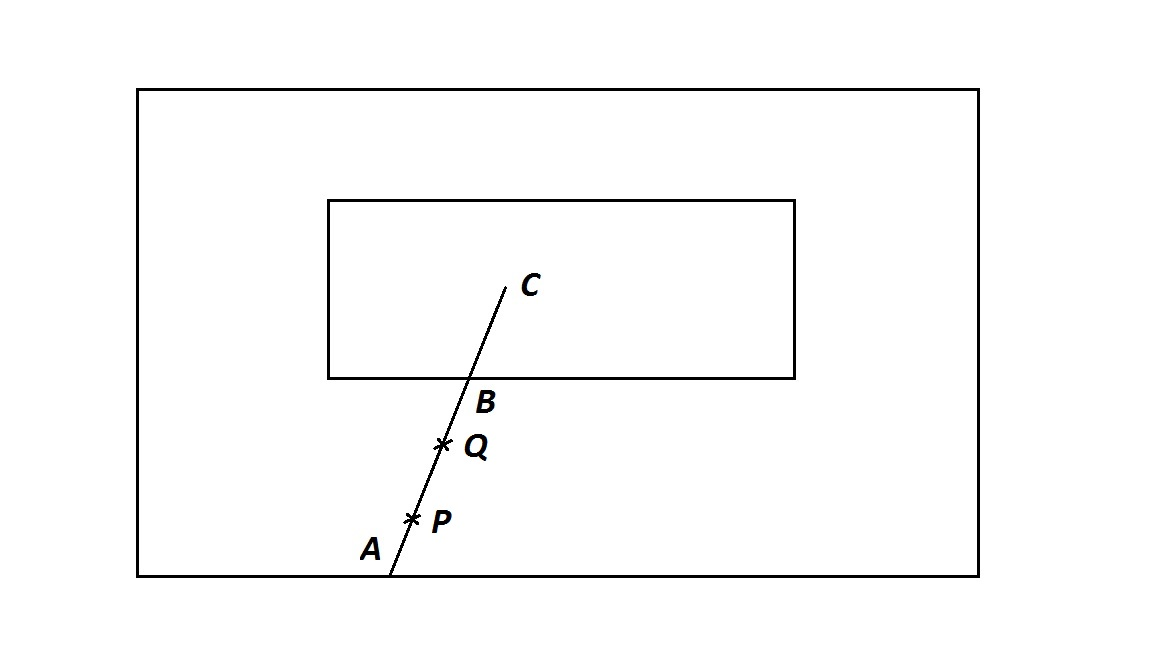
\includegraphics[width=10cm]{transform.jpg}
\centering
\caption{Figure that visualizes the transformation}
\end{figure}

The transformation is visualized in the figure above. A point $C$ is initially decided in the obstacle. The point $C$ needs to be able to see all other points in the obstacle. Then a line is draw from inside the obstacle to the boarder of the part of the map. Because of the law of similarity, the following equation holds:
$$
\frac{AC}{BC} = \frac{PC}{QC}
$$
Here $P$ is a point on the map with an obstacle and $Q$ is the corresponding point on the map without obstacle. In this way, all points except the singular point $C$ can be transformed between these two maps according to the equation above. 

There is a method to handle the singularity point in the article \cite{noncov}, which suggests giving a weight to the cells that represent the obstacles. With these weights, the centroid can be moved to a new location than $C$. But the method assumes a very small weight which can cause numerical error. Instead another method is applied, which is to move the centroid to a new location directly without adding weight. This method will not give the fine properties described in \cite{noncov}, for example arbitrary small errors. But this method is easier to implement and the results are satisfying for our problem. 


\subparagraph{Weight function}
The weight function is a modified Gaussian distribution function. the function will assign a weight between $0$ and $1$ for each cell. Since the pursuers should search locations that haven't been searched instead of staying at one spot with good vision, the weight function needs to change with time. The change is empirically decided as follows: 
\begin{equation}
\begin{split}
d & = \textrm{distance between the cell (i,j) and the nearest pursuer} \\
t_{missing} & = \textrm{time since the evader went missing} \\
\sigma & = t_{missing}^{0.1} \\
W(i, j) & = 1-\frac{1}{\sqrt{2 \pi \sigma}} e^{-\frac{d^2}{2\sigma}}+0.001 \\ 
W_p(i, j) & = 
\begin{cases}
W(i, j)\times t_{missing}^{0.1} & \textrm{, if cell (i, j) is not observable} \\
W(i, j)\div t_{missing}^{0.1} & \textrm{, if cell (i, j) is observable} \\
\end{cases}
\end{split}
\end{equation}
The exponent $0.1$ is decided empirically to avoid rapidly increasing weight. The purpose of the number $0.001$ is to avoid numerical error when calculating the centroid. 

These formulas means that the weight of the cells that are not observable is close to $1$ and increasing with time and distance from the pursuers. And the cells that are observable has lower weight and decreases with time. This will keep the pursuer motivated to keep searching if the evader is not found. 

\subsubsection{Chasing}
The chasing begins when the evader is found. When at least one pursuer sees the evader, all of the pursuers will change it's target to the current location of the evader and begin to chase it. 

\paragraph{Implementation}
Chasing is simply done by the virtual vehicle approach discussed in the open space problem. When the target points are decided, a straight path is automatically presented in the transformed map as the line segment between the pursuers and evader. Then the line segment is inverse-transformed back to a curve in the map with obstacles. The new curve is now seen as reference path the pursuer wants to follow. The $s$ parameter is chosen as the distance traveled on the reference path. So the following control parameters are used:
$$
u = \frac{v_e}{\sqrt{p'^2(s)+q'^2(s)}} 
$$
$v_e$ is the velocity of the corresponding agent and other parameters are previously defined in the Virtual Vehicle Approach section. 


\subsubsection{Re-searching when the evader goes missing}
When the evader goes missing, a strategy is needed for the pursuer to locate it again. Two strategies are empirically chosen and studied. 
\paragraph{The old weight function}
This strategy means to go back to the weight function  and do the search again as soon as the evader is hiding. 
\paragraph{Search the location of last appearance}
When the evader goes missing, all pursuers continue to move toward to the place where the evader was last time seen, until at least one of them goes in a certain range of that location. If no evader is found, the pursuers go back to the weight function strategy and restart the search. 

\subsection{Evading strategy}
In the lack of time and better ideas, only two strategies are chosen for the evader. One of them is the coverage control with weight function, same idea from \cite{sui}. The other one is to predefine several hiding spots. The evader always tries to move to the furthest hiding spot from the nearest pursuer. 

\subsubsection{Weight function}
The coverage control method for the evader is the same as for the pursuer. The only difference is the weight function. Since the closer to the evader the safer the location is for the evader to move to, the weight function should decrease with distance from the evader. Since the evader does not know exactly how far the pursuers can see, it must always assume that the pursuers have infinite long line of sight. Then the weight function become: 
\begin{equation}
\begin{split}
d & = \textrm{distance between the cell (i,j) and the nearest pursuer} \\
t_{missing} & = \textrm{time since the evader went missing} \\
\sigma & = t_{missing}^{0.2} \\
W(i, j) & = \frac{1}{\sqrt{2 \pi \sigma}} e^{-\frac{d^2}{2\sigma}}+0.001 \\ 
W_p(i, j) & = 
\begin{cases}
W(i, j)\times t_{missing}^{0.2} & \textrm{, if cell (i, j) is not observable} \\
W(i, j)\div t_{missing}^{0.2} & \textrm{, if cell (i, j) is observable} \\
\end{cases}
\end{split}
\end{equation}
Then the same procedure will be performed. 

\subsubsection{Hiding spots method}
The observable hiding locations are initially decided assuming infinite long sight of the pursuer. Then the evader moves to the hiding spot with the strategy described above. The hiding spots are decided before the simulation. The idea behind chosing some hiding spots over others is that these locations are harder to locate which means easier to hide. The numerical implementation is done by iteration through a list that contains the hiding spots, and by choosing the best one according to the criteria above.


\chapter{Simulation parameters and the simulation results}

\section{Open space}
The parameters for the numerical simulation are influenced by the parameters for a regular house mouse and a normal human being. The human being the pursuer and the mouse being the evader. It is difficult to acquire the precise number of the parameters that describe their separate dynamics which is why some parameters are accurately estimated. 
The maximum velocity of the mouse is $3 m/s$ and for the human $4 m/s$. The maximum acceleration of the mouse is $6 m/s^2$ and for the human $5 m/s^2$. The maximum angular velocities of the mouse and human are $21 s^{-1}$ and $8 s^{-1}$. The maximum angular acceleration of the mouse and the human are $550 s^{-2}$ and $30 s^{-2}$. The data is acquired from these sources \cite{kinhuman}, \cite{kinmouse} and modified slightly for this experiment. 
The initial position is decided beforehand and some pursuers have none-zero initial velocity at varied directions in order to compare strategies. The detailed information of initial positions can be found in our simulation code. \cite{code}

\subsection{Simulation results}
\subsubsection{Random walk}
Since the randomized walking strategy generates random simulation results, several of those are presented. 

\begin{figure}[H]
\centering
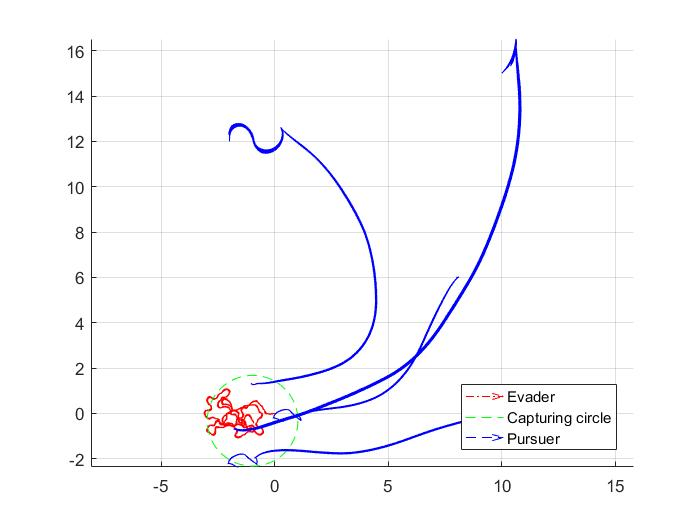
\includegraphics[scale=0.35]{open_random_easy}
\caption{Situation when the evader is caught easily. Catch at $5.7 s$}
\end{figure}

\begin{figure}[H]
\centering
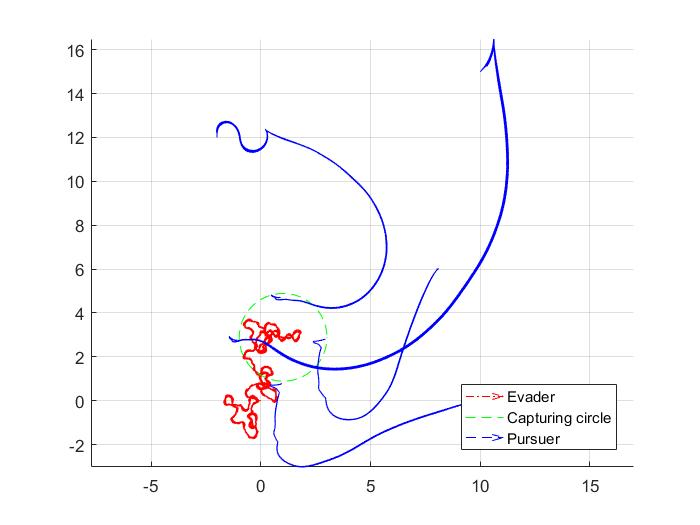
\includegraphics[scale=0.35]{open_random_easy2}
\caption{Another situation when the evader is caught easily. Catch at $6.7 s$}
\end{figure}

\begin{figure}[H]
\centering
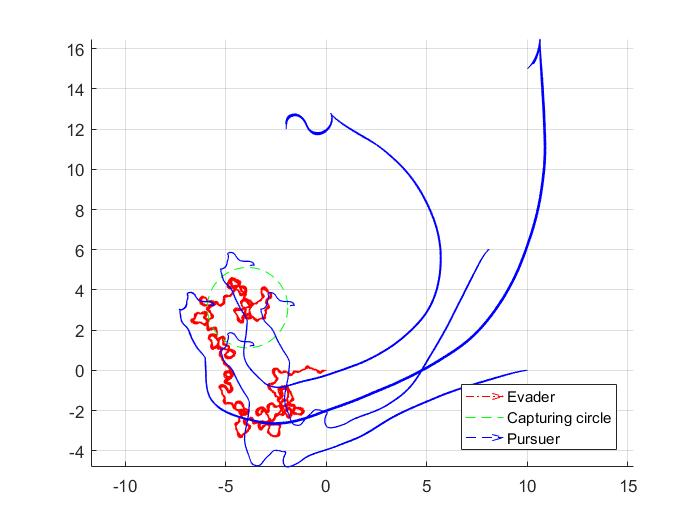
\includegraphics[scale=0.35]{open_random_medium}
\caption{When the catching is more troublesome. Catch at $17.7 s$}
\end{figure}

\begin{figure}[H]
\centering
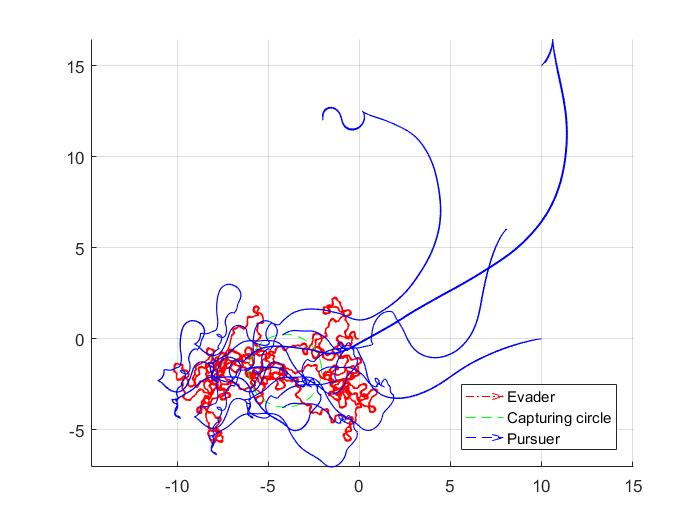
\includegraphics[scale=0.35]{open_random_complex}
\caption{A really difficult catch. Catch at $55.6 s$}
\end{figure}

\subsubsection{Spiral path}
\begin{figure}[H]
\centering
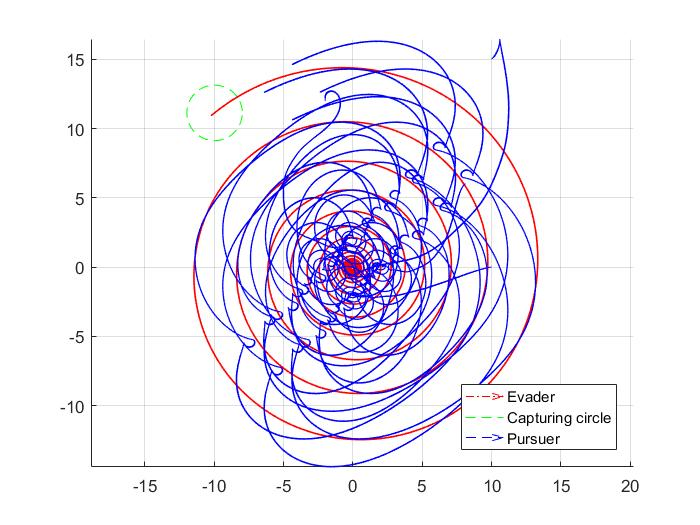
\includegraphics[scale=0.35]{open_spiral_path}
\caption{The spiral strategy. Evader escapes, $100 s$}
\end{figure}

\subsubsection{Periodical path}
\begin{figure}[H]
\centering
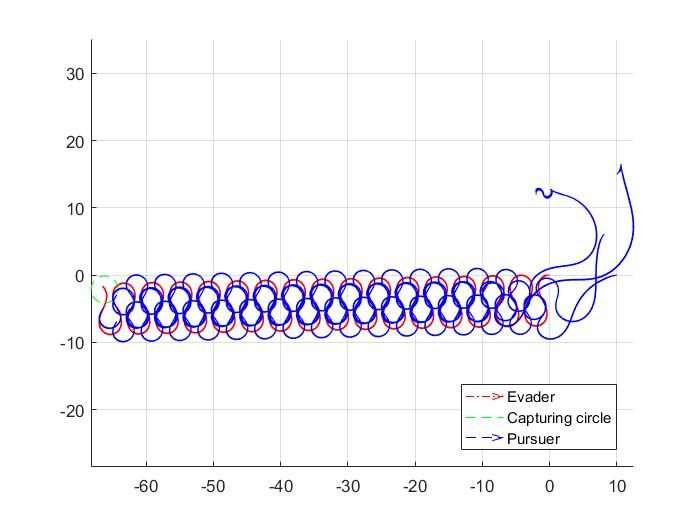
\includegraphics[scale=0.35]{open_periodic_path}
\caption{The periodical strategy. Evader escapes, $100 s$}
\end{figure}


\subsubsection{A complex path for comparison}
\begin{figure}[H]
\centering
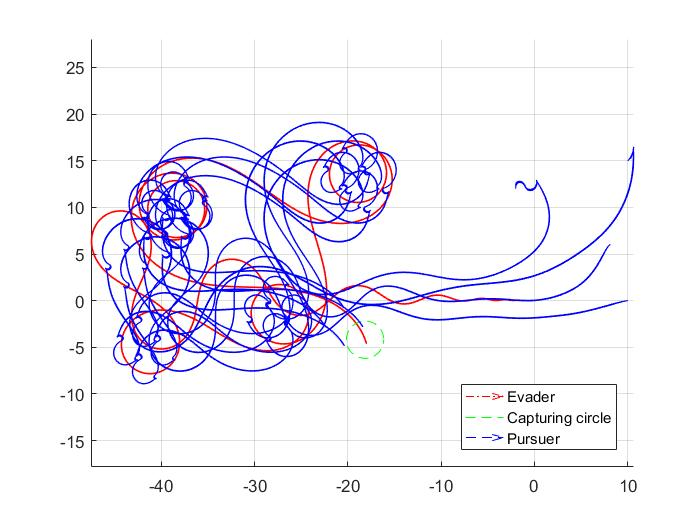
\includegraphics[scale=0.35]{open_complex_path_for_comparison}
\caption{The complex path. Evader escapes, $100 s$}
\end{figure}


\section{Closed space}
The maximum velocities of the pursuer and the evader are $0.5$ and $0.4$. The unit is irrelevant and the time parameter is simplified to integer time steps. The initial location of the pursuer and the evader and the location of the obstacles are shown in the figure below. 

\begin{figure}[H]
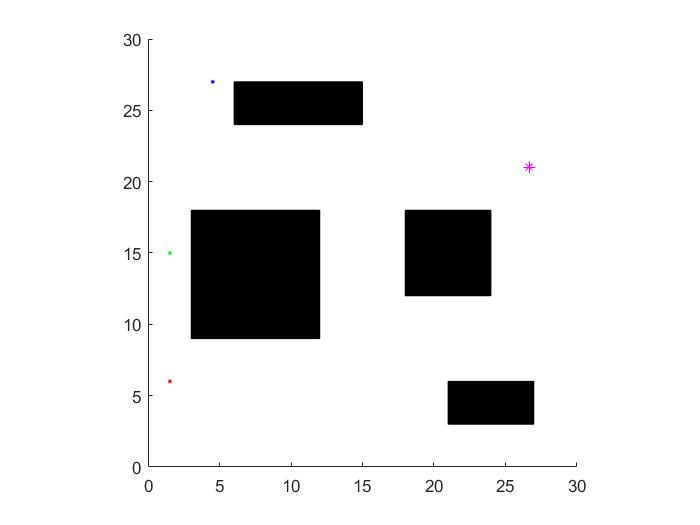
\includegraphics[scale=0.4]{obstacles}
\centering
\caption{The appearance of the initial map.}
\end{figure}

The red, green and blue dots represent the pursuers and the purple star is the evader. The black shapes represent the obstacles. The border of the map is not drawn but assumed to be the boarder of this plot. 

\subsection{Simulation results}


\subsubsection{Case 1}
This is the simulation result when the pursuers return to search with the coverage control algorithm as soon as the evader goes missing. The evader uses the strategy of moving to the furthest hiding spot. 

\begin{figure}[H]
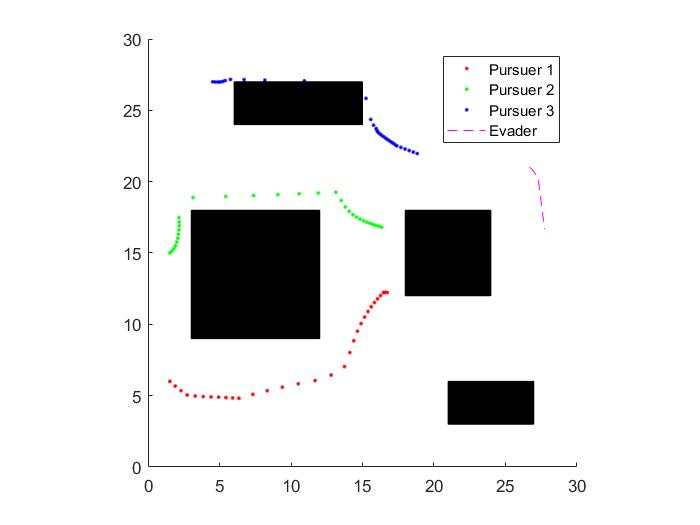
\includegraphics[scale=0.4]{c1-1}
\centering
\caption{The evader is observed and the chasing begins.}
\end{figure}

\begin{figure}[H]
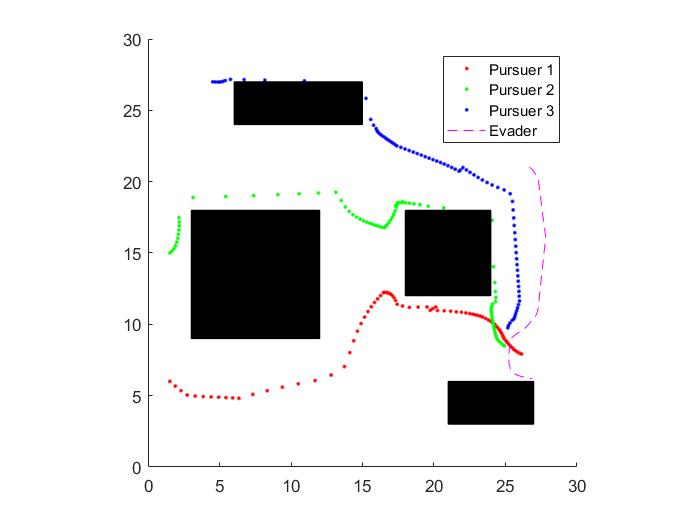
\includegraphics[scale=0.4]{c1-2}
\centering
\caption{The evader tries to hide.}
\end{figure}

\begin{figure}[H]
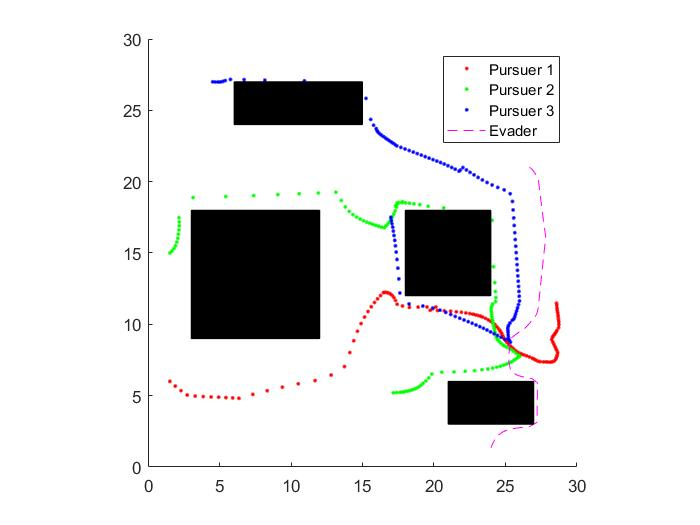
\includegraphics[scale=0.4]{c1-3}
\centering
\caption{The evader goes missing and the search restarts.}
\end{figure}

\begin{figure}[H]
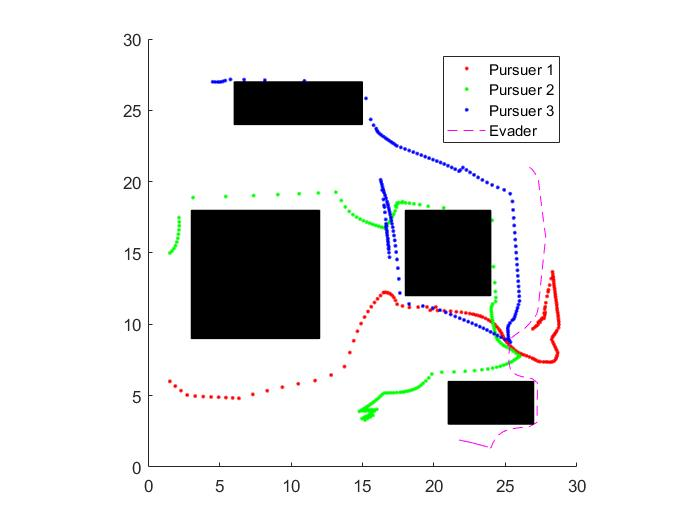
\includegraphics[scale=0.4]{c1-4}
\centering
\caption{The evader is observed again and the chase begins.}
\end{figure}

\begin{figure}[H]
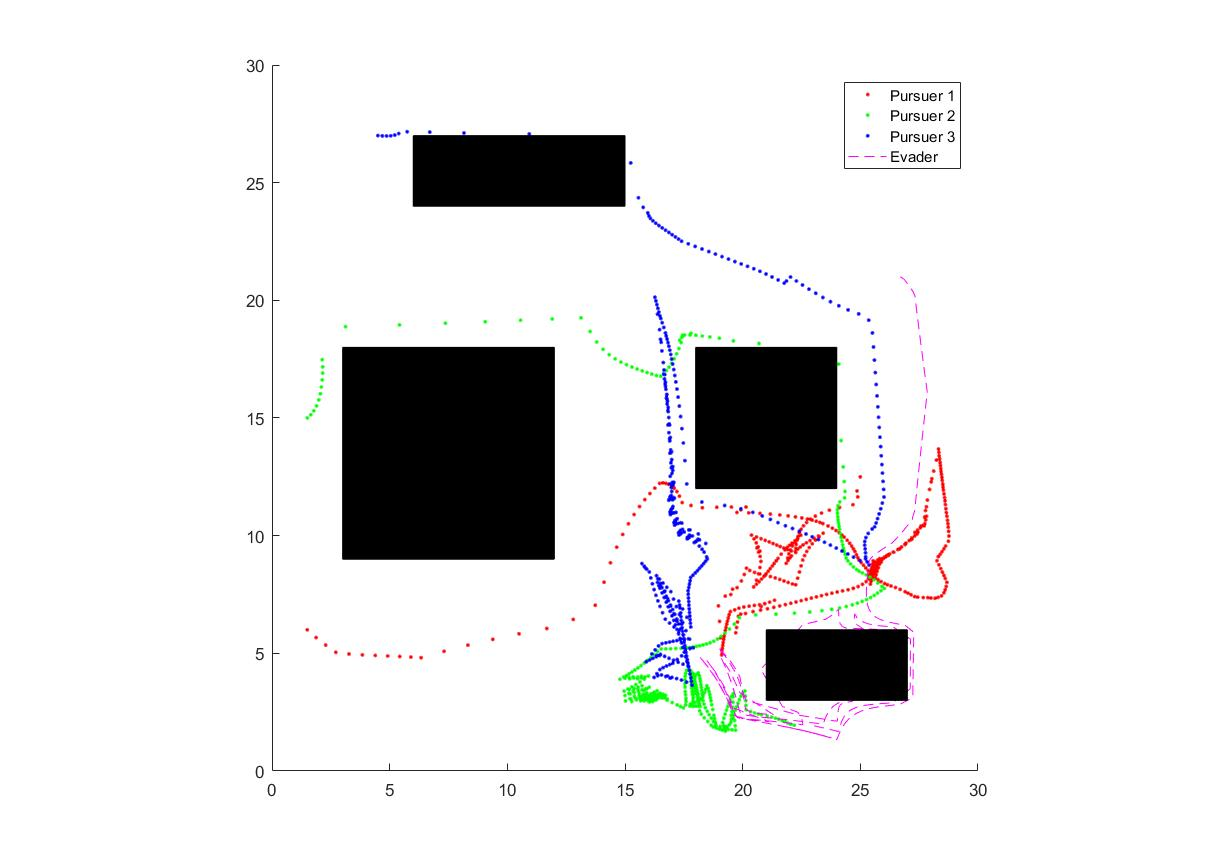
\includegraphics[scale=0.4]{c1_fin}
\centering
\caption{The final result, the evader is caught after 2106 time units.}
\end{figure}

\subsubsection{Case 2}
The pursuers continue to the last appearance location and the evader moves toward the hiding spots.

\begin{figure}[H]
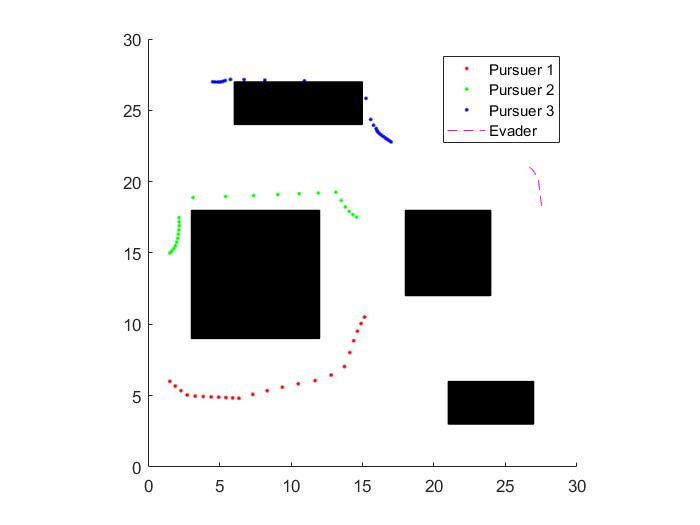
\includegraphics[scale=0.4]{close_second}
\centering
\caption{The evader is observed and the chasing begins.}
\end{figure}

\begin{figure}[H]
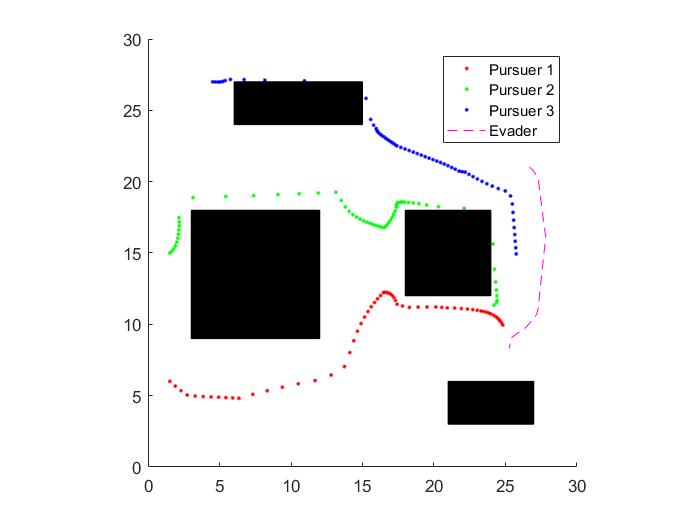
\includegraphics[scale=0.4]{close_third_chase}
\centering
\caption{The evader is running away and the pursuers are chasing.}
\end{figure}

\begin{figure}[H]
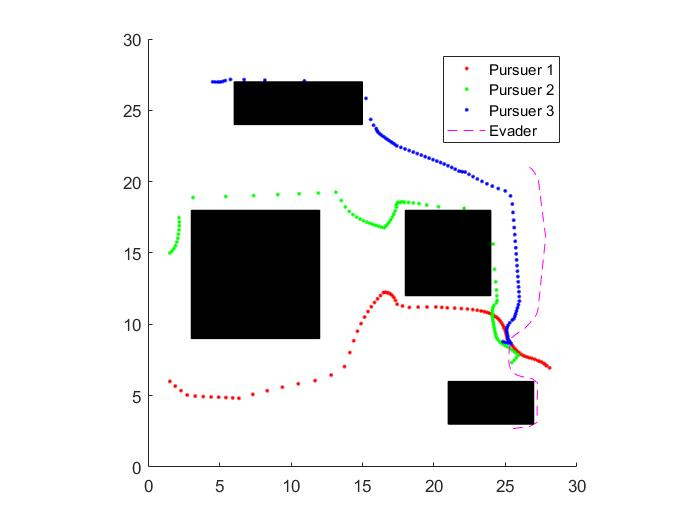
\includegraphics[scale=0.4]{close_fourth_hide}
\centering
\caption{The evader successfully hides.}
\end{figure}

\begin{figure}[H]
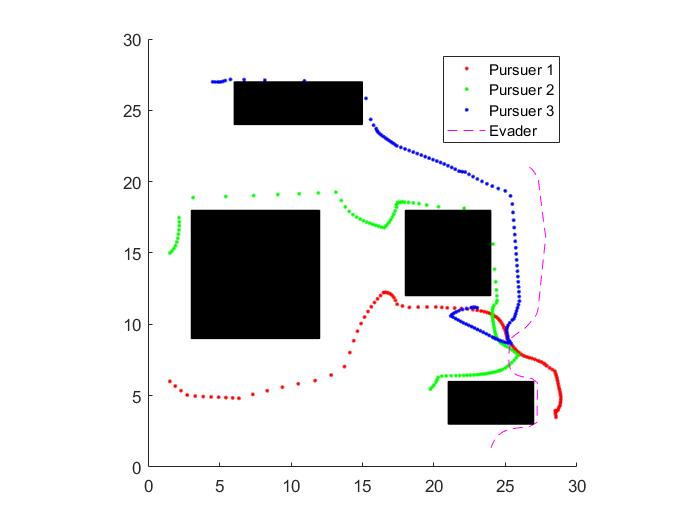
\includegraphics[scale=0.4]{close_fifth_search_again}
\centering
\caption{The pursuers continues to the location where the evader last appeared.}
\end{figure}

\begin{figure}[H]
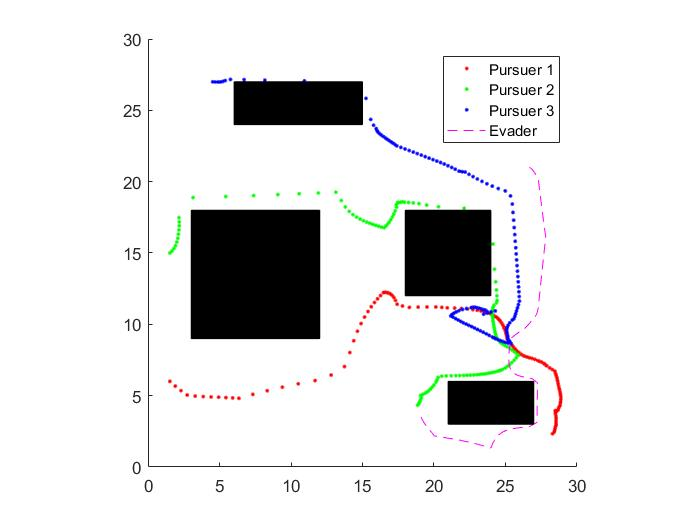
\includegraphics[scale=0.4]{close_finished}
\centering
\caption{The evader is forced to run again and is caught by a pursuer. The final time is 651 time units.}
\end{figure}

\subsubsection{Case 3}
The pursuers use the last-appearance method and the evader only uses the coverage control strategy. 

\begin{figure}[H]
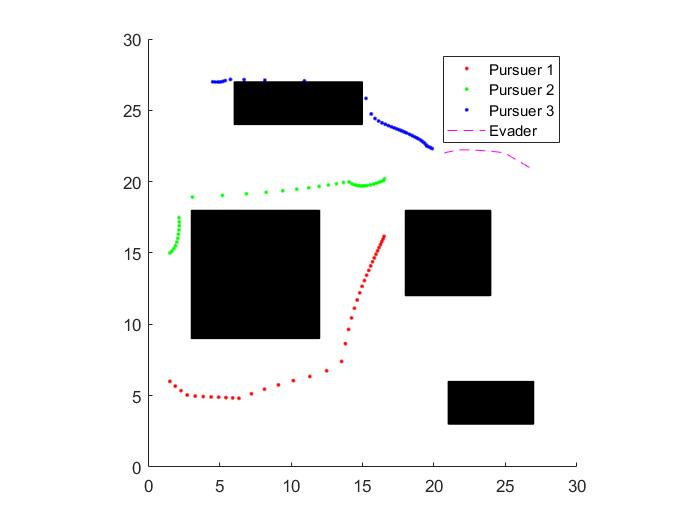
\includegraphics[scale=0.4]{stupid_evader}
\centering
\caption{The evader is moving straight into the pursuers. The process ended after 186 time units. }
\end{figure}

Since the evader never hides in this case when the coverage control strategy is applied, there is no difference which strategy the pursuers use. 

\chapter{Discussion and analysis}

\section{Open space}
The results of the randomized walking strategy varies greatly which is expected. However all of the presented results and most tested cases shows that the evader will be caught if it moves randomly. 

But when the evader tries to leave the map in a slightly more complex path, the pursuers will have some trouble catching it. It is not too difficult to understand since the angular acceleration of the evader is more than 10 times greater than the pursuers. Even if the maximum velocity of the evader is less than the pursuers, it is shown being not too helpful. This is due to the pursuers wasting a lot of its velocity in changing moving direction instead of chasing. This can be seen in figure 3.7, complex path for comparison. Even though the evader does not move too far away from the center of the map, the pursuers can't follow up on its direction changes. 

Since two out of four agents have an initial velocity in a certain direction, this makes it necessary for the agents in most of the randomized simulation cases to make sharp turns. The agents who do not have an initial velocity follow a more effective trajectory that takes less time in regards to catching the evader. While on the contrary the other two agents follow a more realistic path in regards to reacting time, which is something that has to be considered. 

\section{Closed space}
The best strategy for the pursuers is clearly when the last appearance location is considered. It can be seen from the figure that if it is not considered, the pursuers won't go bother checking the most likely spot for the evader to be in. Even after a short period of time if the evader is found again, they will have to run all the way back. This is clearly not optimal and this is why this last-appearance location is introduced. 

As for the strategy of the evader, the coverage control is an incomplete idea. The idea behind the coverage control is good since it works fine with the pursuers. But there is a problem with it. Since there is only one evader, the centroid can possibly be located behind the pursuers. This means that the evader will have to move through a group of pursuers to reach the best location on the map. This is clearly not optimal. A better path design method is needed to work with the coverage control method. 

Since the acceleration is assumed to be infinite, going forward and backwards to increase the chasing time is not a bad idea but this does not happen with the hiding-spots method. So this method is clearly suboptimal as well. 


\section{Overall achievement}
Through out the article working solutions of multiple pursuers-evader is designed. Different solutions are compared and analyzed. A working simulation code is programmed. 

\section{Possible improvement}
\paragraph{Better regulator in the open space}
In the open space, the moving direction of the pursuers varies a lot. With a better designed regulator the pursuers could be able to run in a better pattern. A possible choice is a PID regulator instead of a simple P regulator. 

\paragraph{Better chasing strategy in the open space}
The pursuers move straight towards the evader without planning ahead where the evader will end up. This is clearly not the most intelligent behaviour. A better strategy would be to let the pursuers form a circle with a large radius which encircle  the evader. When the evader is encircled, decrease the radius until caught. 

\paragraph{Better method for computing the field of sight}
The method of computing the line of sight is not very precise and is not very fast. Perhaps with computational geometrics, this can be improved. 

\paragraph{Better chasing strategy in the close space}
The pursuers see obstacles only as something to avoid but not as a help to block the evader from taking certain paths. With a strategy that takes this into account the pursuing can be optimized greatly. 

\paragraph{Better evading strategy in the close space}
As mentioned above, none of the applied strategies are close to optimal. Better idea of strategy is needed. 

\chapter{Appendix}
\listoffigures
\begin{thebibliography}{9}

\bibitem{111}

J von Neumann, O. Morgenstern, \emph{The Theory of Games and Economic Behavior}. Princeton University Press, 1944.

\bibitem{222}

A. H. Copeland, \emph{"Review: Theory of Games and Economic Behavior by John von Neumann and Oskar Morgenstern"}, 1945.

\bibitem{333}

R. Isaacs, Differential Games:  \emph{Mathematical Theory with Applications to Warfare and Pursuit, Control and Optimization}, John Wiley \& Sons, New York, 1965



\bibitem{vva}
  	M. Egerstedt, Xiaoming Hu, and A. Stotsky,
  	\emph{Control of Mobile Platforms Using a Virtual Vehicle Approach},
	IEEE TRANSACTIONS ON AUTOMATIC CONTROL, 
    VOL. 46, NO. 11, 
    NOVEMBER 2001
    
\bibitem{sui}
	David A. Anisi, Petter \"{O}gren and Xiaoming Hu
	\emph{Cooperative Minimum Time Surveillance With Multiple Ground Vehicles}
    IEEE TRANSACTIONS ON AUTOMATIC CONTROL, 
    VOL. 55, NO. 12, 
    DECEMBER, 2010
  
    
\bibitem{cov}
	Jorge Cort\'{e}s, Sonia Mart\'{i}nez, Timur Karatas, Francesco Bullo
	\emph{Coverage control for mobile sensing networks}
    IEEE TRANSACTIONS ON ROBOTICS AND AUTOMATION 
    DECEMBER, 2002

\bibitem{noncov}
	Carlos Humberto Caicedo-N\'{u}\~{n}ez and Milo\v{s} \v{Z}efran
	\emph{A coverage algorithm for a class of non-convex regions}
    Proceedings of the 47th IEEE Conference on Decision and Control
	Cancun, Mexico, 
    DECEMBER 9-11, 2008
    
\bibitem{perfcov}
	Carlos Humberto Caicedo-N\'{u}\~{n}ez and Milo\v{s} \v{Z}efran
    \emph{Performing coverage on nonconvex domains}
    17th IEEE International Conference on Control Applications 
    Part of 2008 IEEE Multi-conference on Systems and Control
    San Antonio, Texas, USA, SEPTEMBER 3-5, 2008
    
  
\bibitem{line}
	Colin Flanagan
    \emph{The Bresenham Line-Drawing Algorithm}
	\url{https://www.cs.helsinki.fi/group/goa/mallinnus/lines/bresenh.html}
    MAY, 2017    
    
\bibitem{kinhuman}
	Brendan Burkett
    \emph{Basic principles for understanding sport mechanics}
    \url{http://www.humankinetics.com/excerpts/excerpts/basic-mechanical-principles}
    
\bibitem{kinmouse}
	Rebecca M. Walter
    \emph{Kinematics of $90^o$ running turns in wild mice}
    The Journal of Experimental Biology 206, 1739-1749
    27 February 2003 
    
\bibitem{code}
	Yue Jiao
    \emph{Simulation code for this article}
    \url{https://github.com/cleamoon/KTH/tree/master/SA114-KEX}
    May, 2017

\bibitem{gametheory}
	\url{http://www.investopedia.com/terms/g/gametheory.asp}
\bibitem{jas}
	\url{http://www.airforce-technology.com/projects/gripen/}
\bibitem{bbc}
	\url{http://www.bbc.com/news/magazine-31503875}
\bibitem{pandm}
	\url{https://en.wikipedia.org/wiki/Princess_and_Monster_game}



    
    
\end{thebibliography}

\end{document}
\endinput














